\documentclass[12pt]{article}

\usepackage{geometry}
\usepackage{fancyhdr}
\usepackage{pifont}
\usepackage{graphicx}
\usepackage{mathrsfs}

\usepackage{fancyhdr}
\usepackage{extramarks}
\usepackage{amsmath}
\usepackage{amsthm}
\usepackage{amsfonts}
\usepackage{tikz}
\usepackage[plain]{algorithm}
\usepackage{algpseudocode}
\usepackage{ctex}


\CTEXoptions[today=old]

\usetikzlibrary{automata,positioning}

%
% Basic Document Settings
%

\topmargin=-0.45in
\evensidemargin=0in
\oddsidemargin=0in
\textwidth=6.5in
\textheight=9.0in
\headsep=0.25in

\linespread{1.3}

\pagestyle{fancy}
\lhead{\hmwkAuthorName}
\chead{\hmwkClass\ : \hmwkTitle}
\rhead{\firstxmark}
\lfoot{\lastxmark}
\cfoot{\thepage}

\renewcommand\headrulewidth{0.4pt}
\renewcommand\footrulewidth{0.4pt}

\setlength\parindent{2em}

%
% Create Problem Sections
%

\newcommand{\enterProblemHeader}[1]{
    \nobreak\extramarks{}{Problem \arabic{#1} continued on next page\ldots}\nobreak{}
    \nobreak\extramarks{Problem \arabic{#1} (continued)}{Problem \arabic{#1} continued on next page\ldots}\nobreak{}
}

\newcommand{\exitProblemHeader}[1]{
    \nobreak\extramarks{Problem \arabic{#1} (continued)}{Problem \arabic{#1} continued on next page\ldots}\nobreak{}
    \stepcounter{#1}
    \nobreak\extramarks{Problem \arabic{#1}}{}\nobreak{}
}

\setcounter{secnumdepth}{0}
\newcounter{partCounter}
\newcounter{homeworkProblemCounter}
\setcounter{homeworkProblemCounter}{1}
\nobreak\extramarks{Problem \arabic{homeworkProblemCounter}}{}\nobreak{}

\newenvironment{homeworkProblem}{
    \section{Problem \arabic{homeworkProblemCounter}}
    \setcounter{partCounter}{1}
    \enterProblemHeader{homeworkProblemCounter}
}{
    \exitProblemHeader{homeworkProblemCounter}
}

%
% Homework Details
%   - Title
%   - Due date
%   - Class
%   - Section/Time
%   - Instructor
%   - Author
%

\newcommand{\hmwkTitle}{Homework\ \#23}
\newcommand{\hmwkDueDate}{\today}
\newcommand{\hmwkClass}{Abstract algebra}
\newcommand{\hmwkClassTime}{Student Number: 518070910121}
\newcommand{\hmwkClassInstructor}{Professor Pu Zhang}
\newcommand{\hmwkAuthorName}{Zixing Wang}

%
% Title Page
%

\title{
    \vspace{2in}
    \textmd{\textbf{\hmwkClass: \hmwkTitle}}\\
    \normalsize\vspace{0.1in}\small{Finished\ on\ \hmwkDueDate\ }\\
   \vspace{0.1in}\large{\textit{\hmwkClassInstructor}}
    \vspace{1in}
\begin{figure}[htb] 
 \center{
\includegraphics[width=5cm]  {DNA.png}} 
 \end{figure}
}

\author{\textbf{\hmwkAuthorName}}
\date{\hmwkClassTime}

\renewcommand{\part}[1]{\textbf{\large Part \Alph{partCounter}}\stepcounter{partCounter}\\}

%
% Various Helper Commands
%

% Useful for algorithms
\newcommand{\alg}[1]{\textsc{\bfseries \footnotesize #1}}

% For derivatives
\newcommand{\deriv}[1]{\frac{\mathrm{d}}{\mathrm{d}x} (#1)}

% For partial derivatives
\newcommand{\pderiv}[2]{\frac{\partial}{\partial #1} (#2)}

% Integral dx
\newcommand{\dx}{\mathrm{d}x}

% Alias for the Solution section header
\newcommand{\solution}{\textbf{\large Solution}}

% Probability commands: Expectation, Variance, Covariance, Bias
\newcommand{\E}{\mathrm{E}}
\newcommand{\Var}{\mathrm{Var}}
\newcommand{\Cov}{\mathrm{Cov}}
\newcommand{\Bias}{\mathrm{Bias}}

\begin{document}

\maketitle
\pagebreak

\begin{homeworkProblem}
1.试构作一个8元域,并写出它的加法表和乘法表
    \par   \noindent   \textbf{Solution}\\
\indent 
$8=2^3$,设F是8元域,则$F$的素域是$\mathbb{Z}_2$,$[F:\mathbb{Z}_2]=3$,找一个$\mathbb{Z}_2$上的3次不可约多项式,比如$f(x)=x^3+x+1$,设$u$是它的一个根,那么$\mathbb{Z}_2(u)$就是一个8元域。

那么计算可得该8元域的元素满足

$
\begin{aligned}
&0=0\\
&u=u\\
&u^2=u^2\\
&u+1=u^3\\
&u^2+u=u^4\\
&u^2+u+1=u^5\\
&u^2+1=u^6\\
&1=u^7
\end{aligned}
$

这些式子给出了乘法的法则。

加法只需要各个系数按照$\mathbb{Z}_2$的加法方式相加即可。

加法表:
\begin{figure}[htb] 
 \center{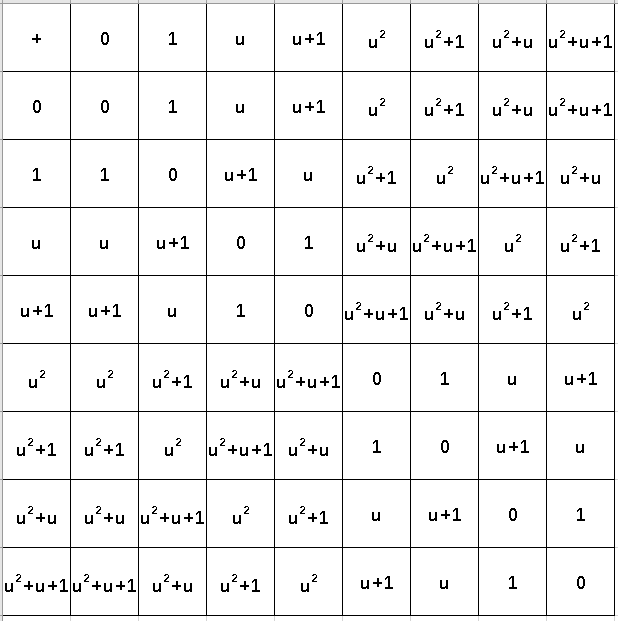
\includegraphics[width=10cm]  {fig1.png}} 
 \end{figure}

乘法表:
\begin{figure}[htb] 
 \center{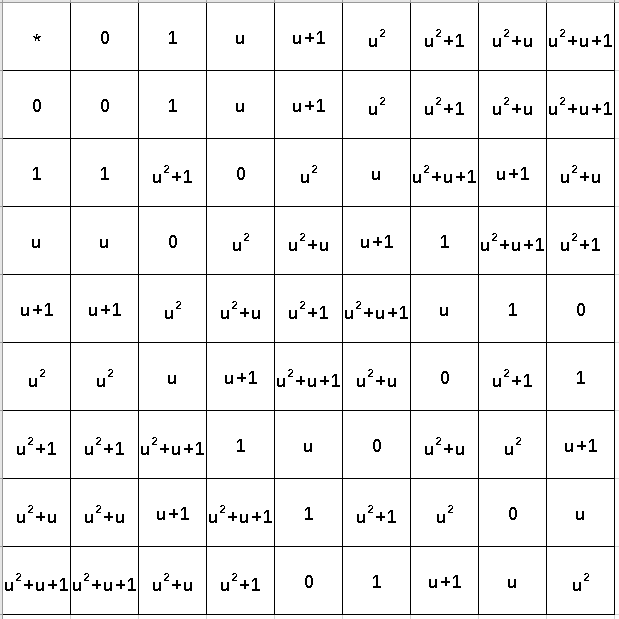
\includegraphics[width=10cm]  {fig2.png}} 
 \end{figure}
\end{homeworkProblem}
\pagebreak

\begin{homeworkProblem}
3. 设 F 为 $p^{n}$ 元域( $p$ 为素数) $, F=F_{p}(u) .$ 试问 $u$ 是否一定为乘法循环群$F^{*}=F-\{0\}$ 的生成元?
    \par   \noindent   \textbf{Solution}\\
\indent
不一定的。

$x^2+1$在$\mathbb{Z}_3[x]$中是不可约多项式。令$u$是方程$x^2+1\in\mathbb{Z}_3[x]$的一个根,因为$u^4=(u^2)^2=2^2=1$,所以在$\mathbb{Z}_3(u)$中$u$不是乘法循环群的生成元。
\end{homeworkProblem}
\pagebreak

\begin{homeworkProblem}
4. 设 $f(x)$ 是 $F_{p}[x]$ 中首 1 不可约多项式.

(1) 若 $u$ 为 $f(x)$ 的一个根,则 $f(x)$ 共有 $n$ 个彼此不同的根,并且它们为 $u, u^{p}, u^{p^{2}}, \cdots, u^{p^{n-1}}$

(2) 若 $f(x)$ 的一个根 $u$ 为域 $F=F_{p}(u)$ 的乘法循环群 $F^{*}=F-\{0\}$ 的生成元,则 $f(x)$ 的每个根也都是 $F^{*}$ 的生成元

(3)证明 $F_{p}[x]$ 中 $n$ 次本原多项式共有 $\varphi\left(p^{n}-1\right) / n$ 个,其中 $\varphi(n)$ 是欧拉函数,表示从 $1$ 到 $n$ 的正整数中与 $n$ 互素的正整数个数。
    \par   \noindent   \textbf{Solution}\\
\indent
(1) 根据有限域的结构定理知 $F_{p}$ 中元 $a$ 均满足 $a^{p}=a,$ 

从而对任一正整数 $t (1 \leq t \leq n-1)$ 均有 $a^{p^{t}}=a$,于是$f\left(u^{p^{t}}\right)=(f(u))^{p^{t}}=0$,

即 $u, u^{p}, \cdots, u^{p^{n-1}}$ 均是 $f(x)$ 的根.

假设存在 $u^{p^{i}}=u^{p^{j}} (1 \leq i<j \leq n-1)$ , 那么 $\left(u^{p^{j-i}}-u\right)^{p^{i}}=u^{p^{j}}-u^{p^{i}}=0,$ 那么 $u^{p^{j-i}-1}=1,$ 于是$F_{p}(u)$ 是 $p^{j-i}$ 元域的子域. 但 $F_{p}(u)$ 是 $p^{n}$ 元域. 这导致了矛盾.

从而假设不成立,因此这些根两两不同。

(2) 若 $u$ 是 $F_{p}(u)$ 的乘法群的生成元, 则 $u$ 的乘法阶为 $p^{n}-1 .$ 因为 $p^{t}(1 \leq t \leq n-1)$ 与 $p^{n}-1$ 互素, 故 $u^{p}, \cdots, u^{p^{n-1}}$ 均为 $p^{n}-1$ 阶元, 从而均是循环群 $F_{p}^{*}(u)$ 的生成元, 即 $f(x)$ 的任一根均是 $F_{p}^{*}(u)$ 的生成元.

(3)我们采用“算两次”的方法来证明。 

设 $F_{p}[x]$ 中共有 $t$ 个 $n$ 次本原多项式, 它们均为多项式 $x^{p^{n}}-x$ 的因子. 设 $E$ 是 $x^{p^{n}}-x$ 所有的根作成的 $p^{n}$ 元域, 则 $E$ 的乘法循环群 $E^{*}$ 有 $\varphi\left(p^{n}-1\right)$ 个 生成元. 

由 (2) 知 $F_{p}[x]$ 中每个 $n$ 次本原多项式的所有根均为 $E^{*}$ 的生成元. 而
$E^{*}$ 的任一生成元均是 $F_{p}[x]$ 中某一个 $n$ 次本原多项式的一个根, 因为两个不同的 $n$ 次本原多项式互素, 所以没有相同的根, 从而 $E^{*}$ 共有 $n t$ 个生成元.

所以$nt=\varphi\left(p^{n}-1\right)$,我们得到 $F_{p}[x]$ 中 $n$ 次本原多项式共有 $\varphi\left(p^{n}-1\right) / n$ 个.
\end{homeworkProblem}
\pagebreak

\begin{homeworkProblem}
7. 设 $K$ 是有限域. 求证 : 对每个 $n \geq 1, K[x]$ 中必存在 $n$ 次不可约多项式.
    \par   \noindent   \textbf{Solution}\\
\indent
设这个有限域 $K$ 是 $p^n$ 元域,特征数是$p$。设$F$是$K$所含的素域,则$K$是$F$的$k$次扩域,即$[K:F]=k$.

作$K[x]$中的多项式$x^{p^{kn}}-x$在$K$上的分裂域$E$, 那么$E$恰好由$x^{p^{kn}}-x$的两两互异的$p^{kn}$个根组成.

$F\subset K \subset E$,且$E$是$F$的有限扩域,且$[E:F]=kn$,所以根据望远镜公式$[E:K]=n$.

因为有限域$E$是素域$F$的一个单扩域,所以存在$E$中的元素$u$,使得$E=F(u)$,那么$E=F(u) \subset K(u)  \subset E$,得到$E=K(u)$,于是$[K(u):K]=n$

那么 $u$ 在 $K$ 上的极小多项式就是 $K[x]$ 中的 $n$ 次不可约多项式.

\iffalse 
因为存在 $p^{n^2}$ 元域 $E$ 使得 $E$ 是 $x^{p^{n^2}}-x \in K[x]$ 在 $F_{p}$ 上的分裂域, 且 $E=K(u)$ 

那么 $u$ 在 $K$ 上的极小多项式就是 $K[x]$ 中的 $n$ 次不可约多项式.
\fi
\end{homeworkProblem}
\pagebreak

\begin{homeworkProblem}
8. (1) 证明 $x^{4}+x+1$ 为 $F_{2}[x]$ 中本原多项式

(2) 列出 16 元域 $F_{16}=F_{2}[u]$ 中(唯一的) 4 元子域的全部元素,这里 $u$ 是
$x^{4}+x+1 \in F_{2}[x]$ 的一个根

(3) 求出 $u$ 在$F_{4}$ 上的极小多项式.
    \par   \noindent   \textbf{Solution}\\
\indent
(1)设$u$是它的一个根,那么

$
\begin{aligned}
&u=u\\
&u^2=u^2\\
&u^3=u^3\\
&u^4=u+1\\
&u^5=u^2+u\\
&u^6=u^3+u^2\\
&u^7=u^3+u+1\\
&u^8=u^2+1\\
&u^9=u^3+u\\
&u^{10}=u^2+u+1\\
&u^{11}=u^3+u^{2}+u\\
&u^{12}=u^3+u^{2}+u+1\\
&u^{13}=u^3+u^2+1\\
&u^{14}=u^3+1\\
&u^{15}=1
\end{aligned}
$

因此,按照本原多项式的定义可知$x^{4}+x+1$ 为 $F_{2}[x]$ 中本原多项式.

(2)
$F_{16}=F_{2}[u]$ 中(唯一的) 4 元子域的全部元素是

$F_4=\{0,1,u^5,u^{10}\}=\{0,1,u^2+u,u^2+u+1\}$

(3)
该极小多项式至少是二次的.

根据上述的关系式可以发现$u$满足$x^2+x+u^5=0$,

所以这是$u$ 在$F_{4}$ 上的极小多项式.
\end{homeworkProblem}
\pagebreak
\end{document}
